\normaltrue \difficilefalse \tdifficilefalse
\correctionfalse

%\UPSTIidClasse{11} % 11 sup, 12 spé
%\newcommand{\UPSTIidClasse}{12}

\exer{Parallélépipède percé$\star$ \label{B2:10:41}}
\setcounter{numques}{0}
\UPSTIcompetence[2]{B2-10}
\index{Compétence B2-10}
\index{Parallélépipède}
\ifcorrection
\else
\textbf{Pas de corrigé pour cet exercice.}
\fi

\ifprof
\else
La matrice d'inertie d'un cylindre d'axe $\axe{G}{k}$ de rayon $R$ et de hauteur $H$ et de masse $m$ est donnée en son centre d'inertie par 
$\inertie{G}{1}=\matinertie{A}{A}{C}{0}{0}{0}{\base{i}{j}{k}}$ avec $A=m\left(\dfrac{R^2}{4}+\dfrac{H^2}{12} \right)$ et $C=m\dfrac{R^2}{2}$. 


La matrice d'inertie d'un parallélépipède rectangle de cotés $a$, $b$ et $c$ et de masse $m$ est donnée en son centre d'inertie par 
$\inertie{G}{1}=\matinertie{A}{B}{C}{0}{0}{0}{\base{i}{j}{k}}$ avec $A={m\dfrac{b^2+c^2}{12}}$, $B={m\dfrac{a^2+c^2}{12}}$, $C={m\dfrac{a^2+b^2}{12}}$.

Soit la pièce suivante. 
\begin{figure}[H]
\centering
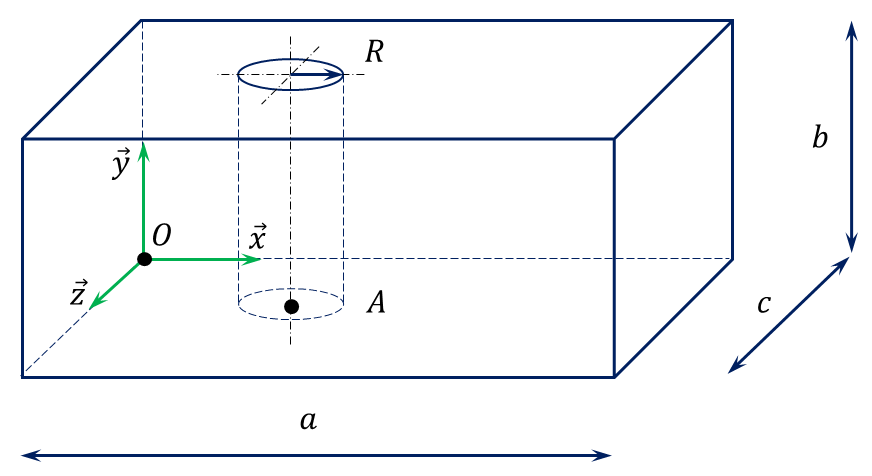
\includegraphics[width=\linewidth]{41_01}
\end{figure}

On pose $\vect{OA}=\dfrac{a}{3}\vect{x}+\dfrac{c}{2}\vect{z}$. 

\fi



\question{Déterminer la position du centre d'inertie $G$ du solide.}
\ifprof
\else
\fi

\question{Déterminer la matrice d'inertie du solide en $G$, en $A$ puis $O$.}
\ifprof ~\\
\else
\fi


\ifprof
\else
\begin{flushright}
\footnotesize{Corrigé voir \ref{B2:10:41}.}
\end{flushright}%
\fi